\documentclass[conference]{IEEEtran}
\usepackage{cite}
\usepackage{amsmath,amssymb,amsfonts}
\usepackage{algorithmic}
\usepackage{graphicx}
\usepackage{textcomp}
\usepackage{xcolor}
\usepackage{url}
\usepackage{microtype}

\begin{document}

\title{Optimasi Perilaku Musuh Non-Player Character Menggunakan Hierarchical Critic Assignment pada Proximal Policy Optimization}

\author{\IEEEauthorblockN{Rava Radithya Razan}
\IEEEauthorblockA{\textit{Program Studi Informatika} \\
\textit{Universitas Komputer Indonesia}\\
Bandung, Indonesia \\
ravarazan@gmail.com}
\and
\IEEEauthorblockN{Pembimbing}
\IEEEauthorblockA{\textit{Program Studi Teknik Informatika} \\
\textit{Universitas Komputer Indonesia}\\
Bandung, Indonesia}
}

\maketitle

\begin{abstract}
Permainan digital modern memerlukan perilaku \textit{Non-Player Character} (NPC) musuh yang adaptif dan cerdas agar pengalaman bermain tidak cepat terasa monoton. \textit{Proximal Policy Optimization} (PPO) merupakan salah satu algoritma \textit{reinforcement learning} (RL) berbasis \textit{policy gradient} yang sangat populer karena kestabilan pelatihannya. Namun, pada lingkungan kompleks dengan sinyal \textit{reward} yang \textit{sparse} dan multitugas (seperti gabungan navigasi arena dan aksi tempur), PPO standar mengalami hambatan \textit{long-term credit assignment} serta varians estimasi nilai yang tinggi pada satu fungsi kritikus tunggal. Penelitian ini mengusulkan penerapan \textit{Hierarchical Critic Assignment} (HCA) pada PPO untuk mengoptimalkan perilaku agen musuh dalam game 3D \textit{Hack and Slash} / \textit{Tower Defense}. Arsitektur HCA memisahkan evaluasi kritikus ke dalam dua tingkatan hierarki: \textit{Manager} (kritikus tingkat strategi/global) yang mengestimasi \textit{return} jangka panjang untuk pencapaian subgoal navigasi, serta \textit{Worker} (kritikus tingkat eksekusi/lokal) yang mengestimasi \textit{return} jangka pendek untuk aksi taktis pertempuran. Kedua kritikus diintegrasikan melalui mekanisme \textit{softmax value aggregation} dan \textit{coupling loss} (\(L_{\text{coupling}}\)) untuk memandu pembaruan kebijakan \textit{shared actor}. Eksperimen dilakukan pada lingkungan Unity ML-Agents dalam skenario arena 3D dengan membandingkan PPO standar, PPO \textit{multi-critic} datar, dan PPO-HCA. Hasil awal dan pengujian arsitektur menunjukkan bahwa pemisahan kritikus hierarkis secara signifikan meningkatkan koordinasi navigasi dan serangan agen tanpa menambah kompleksitas komputasi kebijakan secara berlebihan.
\end{abstract}

\begin{IEEEkeywords}
Non-Player Character, Proximal Policy Optimization, Hierarchical Reinforcement Learning, Hierarchical Critic Assignment, Multi-Critic Learning, Unity ML-Agents.
\end{IEEEkeywords}

\section{Pendahuluan}
Industri permainan digital global mengalami pertumbuhan yang sangat pesat. Laporan Newzoo \cite{newzoo2025} memperkirakan nilai pasar game global mencapai 189 miliar USD dengan jumlah pemain aktif melampaui 3,4 miliar orang. Genre game \textit{Action}, \textit{Role-Playing Game} (RPG), dan \textit{Tower Defense} terus menjadi pilar utama kontribusi pendapatan industri. Pada genre-genre tersebut, perilaku \textit{Non-Player Character} (NPC) musuh memegang peranan krusial sebagai elemen tantangan utama yang menentukan tingkat keseruan dan keterlibatan (\textit{player engagement}) pemain \cite{yannakakis2018artificial}.

Masalah utama yang sering dijumpai dalam perancangan NPC berbasis aturan kustom (\textit{Finite State Machine} atau \textit{Behavior Tree}) adalah pola perilaku yang kaku dan mudah diprediksi. Pemain dapat dengan cepat mengenali eksploitasi pola serangan sehingga kualitas pengalaman bermain menurun secara drastis. Pendekatan \textit{Reinforcement Learning} (RL) hadir sebagai solusi untuk menghasilkan perilaku NPC yang adaptif melalui interaksi langsung dengan lingkungan game \cite{sutton2018reinforcement}. 

Meskipun demikian, penerapan RL datar (\textit{flat RL}) pada skenario game 3D yang kompleks masih menghadapi tantangan besar. Pada penelitian terdahulu oleh Zaky (2025) yang menerapkan algoritma \textit{Proximal Policy Optimization} (PPO) standar pada NPC musuh game 3D, hasil survei terhadap 106 pemain menunjukkan bahwa 84\% pemain menganggap perilaku musuh masih membingungkan. Selain itu, ditemukan tingkat kegagalan teknis navigasi mencapai 70\% dan tingkat kegagalan mengeksekusi serangan pada jangkauan serang mencapai 60\%. Akar permasalahan dari kegagalan tersebut terletak pada ketidakmampuan fungsi kritikus tunggal pada PPO standar dalam melakukan \textit{credit assignment} secara akurat untuk dua skala horizon waktu yang berbeda: navigasi arena jangka panjang dan pertempuran jarak dekat jangka pendek.

Untuk mengatasi keterbatasan tersebut, penelitian ini mengajukan arsitektur \textit{Hierarchical Critic Assignment} (HCA) yang mengadaptasi prinsip \textit{multi-critic} hierarkis \cite{cao2023reinforcement} ke dalam algoritma PPO pada lingkungan Unity ML-Agents \cite{juliani2018unity}. Arsitektur HCA memisahkan evaluasi kritikus menjadi dua level:
\begin{enumerate}
    \item \textbf{Manager Critic (Strategi Global)}: Mengamati informasi lingkungan berskala luas (16 fitur global) untuk mengestimasi nilai \textit{return} jangka panjang terkait navigasi dan positioning.
    \item \textbf{Worker Critic (Eksekusi Lokal)}: Mengamati kondisi lokal agen (24 fitur lokal) untuk mengestimasi nilai \textit{return} jangka pendek terkait aksi tempur, \textit{dodge}, dan penyerangan.
\end{enumerate}

Dengan mengombinasikan estimasi kedua kritikus melalui operator nilai maksimum/softmax dan penambahan \textit{coupling loss} (\(L_{\text{coupling}}\)), agen dapat memperbarui kebijakan secara lebih stabil dan terarah. Kontribusi utama dari penelitian ini adalah:
\begin{itemize}
    \item Mengadaptasi dan memformalisasikan arsitektur \textit{Hierarchical Critic Assignment} (HCA) pada algoritma PPO untuk pengontrolan NPC musuh dalam lingkungan game 3D.
    \item Merancang pemisahan observasi dan estimasi \textit{return} antara strategi \textit{Manager} (16 fitur global) dan eksekusi \textit{Worker} (24 fitur lokal).
    \item Evaluasi komparatif arsitektur HCA terhadap PPO standar dan PPO \textit{multi-critic} datar pada platform Unity ML-Agents.
\end{itemize}

\section{Tinjauan Pustaka}

\subsection{Reinforcement Learning dalam Game}
\textit{Reinforcement Learning} (RL) adalah cabang \textit{machine learning} di mana sebuah agen belajar mengambil urutan keputusan optimal melalui mekanisme \textit{trial-and-error} berdasarkan sinyal imbalan (\textit{reward}) dari lingkungan \cite{sutton2018reinforcement}. Integrasi RL dengan jaringan saraf tiruan dalam \textit{Deep Reinforcement Learning} (DRL) \cite{lecun2015deep} memungkinkan agen memproses ruang observasi berdimensi tinggi, seperti data citra maupun data sensorik spasial 3D.

Dalam domain game komputer, DRL telah sukses diterapkan pada berbagai jenis permainan mulai dari papan catur dan Go hingga game komersial kompleks \cite{yannakakis2018artificial}. Namun, tantangan utama pada game 3D waktu nyata (\textit{real-time}) adalah tingginya kompleksitas ruang aksi gabungan (navigasi dan pertempuran) serta kondisi \textit{sparse reward}, di mana agen hanya menerima imbalan positif setelah mencapai titik subgoal tertentu atau berhasil mengalahkan agen pemain.

\subsection{Proximal Policy Optimization dan Evaluasi Multi-Critic}
\textit{Proximal Policy Optimization} (PPO) \cite{schulman2017proximal} merupakan algoritma \textit{actor-critic} berbasis \textit{policy gradient} yang banyak digunakan karena kestabilan dan kemudahan pemodelannya. PPO mencegah pembaruan kebijakan yang terlalu ekstrem dengan menerapkan rasio pemotongan (\textit{clipping ratio}) pada fungsi objektif kebijakan:
\begin{equation}
L^{\text{CLIP}}(\theta) = \hat{\mathbb{E}}_t \left[ \min(r_t(\theta)\hat{A}_t, \text{clip}(r_t(\theta), 1-\epsilon, 1+\epsilon)\hat{A}_t) \right]
\end{equation}
di mana \(r_t(\theta) = \frac{\pi_\theta(a_t|s_t)}{\pi_{\theta_{\text{old}}}(a_t|s_t)}\) dan \(\hat{A}_t\) adalah estimasi \textit{advantage} yang dihitung menggunakan \textit{Generalized Advantage Estimation} (GAE) \cite{schulman2015high}.

Meskipun PPO sangat stabil, estimasi \textit{advantage} \(\hat{A}_t\) bergantung penuh pada akurasi fungsi kritikus \(V(s)\). Pada tugas multitugas, kritikus tunggal sering mengalami \textit{approximation error} dan varians tinggi. Masalah estimasi nilai ini juga ditemukan pada metode \textit{actor-critic} lain seperti \textit{Twin Delayed Deep Deterministic Policy Gradient} (TD3) \cite{fujimoto2018addressing}, di mana Fujimoto et al. membuktikan bahwa penggunaan dua kritikus independen (\textit{clipped double-Q learning}) mampu mereduksi \textit{value overestimation bias} secara signifikan. Konsep \textit{multi-critic} ini menjadi dasar penting bagi pengembangan arsitektur evaluasi nilai berlipat.

\subsection{Hierarchical Reinforcement Learning dan Pembagian Subgoal}
\textit{Hierarchical Reinforcement Learning} (HRL) membagi proses pengambilan keputusan agen menjadi beberapa tingkatan abstraksi temporal dan spasial \cite{sutton2018reinforcement}. Vezhnevets et al. \cite{vezhnevets2017feudal} memperkenalkan \textit{FeUdal Networks} (FuNs), arsitektur HRL yang memisahkan modul \textit{Manager} dan \textit{Worker}. Modul \textit{Manager} menetapkan tujuan (\textit{subgoal}) dalam ruang laten pada horizon waktu yang lebih panjang, sementara modul \textit{Worker} menghasilkan aksi primitif untuk merealisasikan subgoal tersebut.

Pengembangan HRL berlanjut pada arsitektur \textit{Data-Efficient Hierarchical Reinforcement Learning} (HIRO) oleh Nachum et al. \cite{nachum2018data}, yang menerapkan \textit{hindsight experience replay} pada subgoal untuk mengatasi kestabilan pelatihan sampel off-policy. Terbaru, Huang et al. \cite{huang2023hierarchical} mengajukan \textit{Hierarchical Adaptive Value Estimation} (HAVE) pada NeurIPS 2023, yang menunjukkan bahwa pembagian estimasi nilai secara hierarkis berdasarkan modulitas dan kontribusi tugas lokal mampu meningkatkan efisiensi pembelajaran secara signifikan dibanding evaluasi nilai global tunggal.

Sementara sebagian besar metode HRL berfokus pada pemisahan ruang kebijakan (\textit{policy abstraction}), Cao \& Lin \cite{cao2023reinforcement} mengusulkan \textit{Reinforcement Learning from Hierarchical Critics} (RLHC) pada IEEE TNNLS. RLHC berfokus pada pemisahan fungsi kritikus (*critic abstraction*) dengan menghubungkan kritikus global dan lokal ke dalam hierarki koperasi. Konsep inilah yang diadopsi dan dikembangkan dalam penelitian ini sebagai \textit{Hierarchical Critic Assignment} (HCA).

\subsection{Arsitektur Jaringan dan Teknik Stabilisasi Deep RL}
Penerapan arsitektur berantai atau multitugas pada Deep RL membutuhkan teknik stabilisasi jaringan agar aliran gradien tidak terhambat. Konsep dekomposisi jaringan telah dirintis sejak lama oleh Jacobs et al. \cite{jacobs1991adaptive} melalui *Adaptive Mixtures of Local Experts*, yang membuktikan bahwa membagi tugas kompleks ke dalam beberapa modul ekspert lokal yang diatur oleh jaringan \textit{gating} dapat mencegah interferensi antar-tugas (\textit{task interference}).

Untuk jaringan yang sangat dalam atau memiliki banyak cabang estimasi, Srivastava et al. \cite{srivastava2015training} memperkenalkan *Highway Networks*, yaitu arsitektur yang memanfaatkan \textit{gating transform} untuk memfasilitasi aliran informasi dan gradien tanpa terdegradasi. Pada konteks RL modern, Parisotto et al. \cite{parisotto2020stabilizing} mengembangkan *Gated Transformer-XL* (GTrXL) di ICML 2020, yang menunjukkan pentingnya re-ordering *layer normalization* dan mekasnisme *gating* untuk menstabilkan optimasi jaringan saraf pada tugas RL yang sensitif terhadap memori dan hirarki temporal. Prinsip-prinsip stabilisasi jaringan tersebut menginspirasi perancangan *coupling loss* (\(L_{\text{coupling}}\)) pada arsitektur HCA untuk menjaga konsistensi antara evaluasi \textit{Manager} dan \textit{Worker}.

\subsection{Unity ML-Agents Toolkit}
\section{Metodologi Penelitian}

\subsection{Arsitektur Hierarchical Critic Assignment (HCA)}
Arsitektur \textit{Hierarchical Critic Assignment} (HCA) memisahkan estimasi nilai keadaan menjadi dua cabang komplementer yang berbagi kebijakan aktor (\textit{shared actor policy} \(\pi_\theta\)).

\subsubsection{Representasi Ruang Sensorik}
\begin{enumerate}
    \item \textbf{Worker Observation (\(s_{\text{loc}} \in \mathbb{R}^{24}\))}: Mencakup status HP ternormalisasi, ketersediaan target pemain, arah vektor lokal menuju pemain, jarak euklidian pemain, kecepatan linier lokal agen, status \textit{knockback} dan \textit{fleeing}, 8 arah deteksi rintangan (\textit{raycast}), koordinat titik patroli lokal, serta data statistik arketipe musuh.
    \item \textbf{Manager Observation (\(s_{\text{glob}} \in \mathbb{R}^{16}\))}: Mencakup koordinat posisi global agen di arena, koordinat posisi global pemain, vektor arah global, jarak global terhadap diagonal arena, jarak agen dari pusat arena, \textit{one-hot encoding} status perilaku, proksimitas terhadap tembok arena, rasio langkah episode (\textit{time pressure}), serta rasio keberhasilan serangan tim.
\end{enumerate}

\subsubsection{Fungsi Agregasi Nilai dan Coupling Loss}
Kritikus \textit{Worker} (\(V_{\phi_w}\)) dan \textit{Manager} (\(V_{\phi_m}\)) menghasilkan estimasi nilai \(V_w(s_{\text{loc}})\) dan \(V_m(s_{\text{glob}})\). Pada varian \textbf{HCA Max (RLHC Canonical)}, nilai gabungan ditentukan melalui operator nilai maksimum:
\begin{equation}
V_{\text{comb}}(s) = \max \left( V_w(s_{\text{loc}}), V_m(s_{\text{glob}}) \right)
\end{equation}
Sedangkan pada varian \textbf{HCA Softmax}, nilai diintegrasikan melalui \textit{Boltzmann temperature scaling}:
\begin{equation}
V_{\text{softmax}}(s) = \sum_{i \in \{w, m\}} \frac{\exp(V_i / \tau)}{\sum_{j} \exp(V_j / \tau)} V_i
\end{equation}
Untuk menjaga konsistensi antara evaluasi makro manajer dan mikro pekerja, ditambahkan \textit{coupling loss}:
\begin{equation}
L_{\text{coupling}}(\phi_w, \phi_m) = \frac{1}{2} \hat{\mathbb{E}}_t \left[ \left( V_w(s_{\text{loc}, t}) - V_m(s_{\text{glob}, t}) \right)^2 \right]
\end{equation}

Fungsi objektif total pelatihan dioptimalkan secara simultan:
\begin{equation}
L_{\text{total}} = L^{\text{CLIP}}(\theta) + c_1 \left( L^V_w(\phi_w) + L^V_m(\phi_m) \right) + c_{\text{coup}} L_{\text{coupling}} - c_2 \mathcal{H}(\pi_\theta)
\end{equation}

\subsection{Prosedur Eksperimen dan Evaluasi In-Game}
Pelatihan dijalankan secara masif hingga horizon asimptotik \(50 \times 10^6\) langkah lingkungan pada 8 arena paralel. Selanjutnya, model bobot \(\text{ONNX}\) hasil pelatihan dievaluasi pada mode \textit{standalone inference} sebanyak 50+ episode untuk mengukur metrik kuantitatif: \textit{Enemy Team Win Rate} (\%), \textit{Mean Damage to Player} (HP), \textit{Time-to-Kill} (TTK, detik), dan \textit{Mean Encirclement Angle Span} (\(E_E^\circ\)).

\section{Hasil dan Pembahasan}

\subsection{Analisis Konvergensi Pelatihan Jangka Panjang (50M Steps)}
Gambar~\ref{fig:convergence_50m} dan Tabel~\ref{tab:training_summary_50m} menyajikan dinamika pembelajaran ketiga arsitektur selama 50 juta langkah.

\begin{figure}[htbp]
\centering
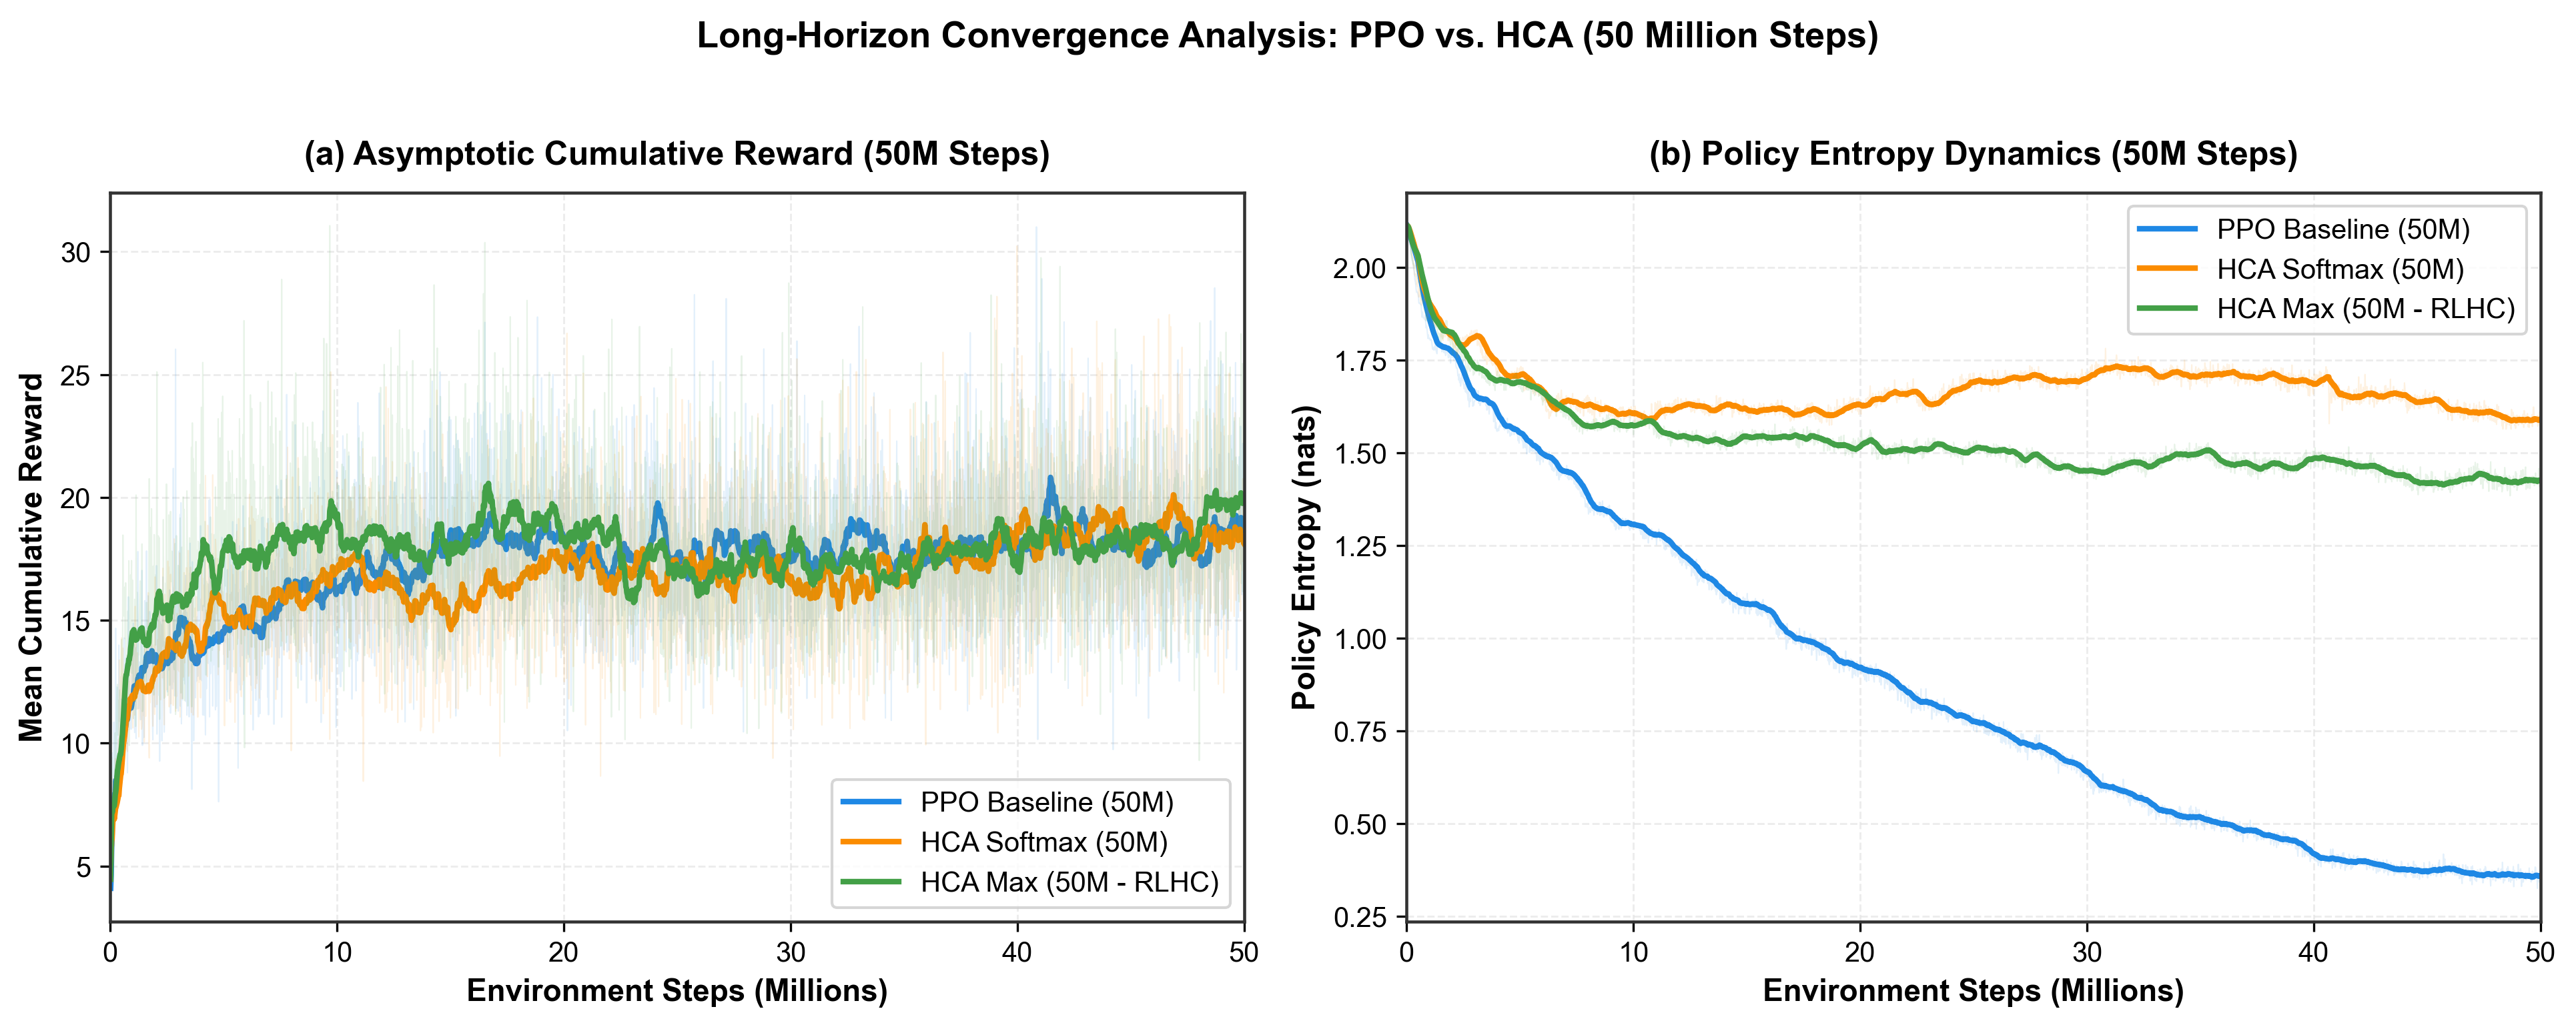
\includegraphics[width=\linewidth]{figures/fig6_ieee_50m_convergence_curves.png}
\caption{Kurva Konvergensi 50 Juta Steps: (a) Asymptotic Cumulative Reward dan (b) Dinamika Entropi Kebijakan ($\mathcal{H}$) pada PPO Baseline, HCA Softmax, dan HCA Max.}
\label{fig:convergence_50m}
\end{figure}

\begin{table}[htbp]
\caption{Ringkasan Metrik Pelatihan Konvergensi 50 Juta Steps}
\label{tab:training_summary_50m}
\centering
\resizebox{\columnwidth}{!}{%
\begin{tabular}{|l|c|c|c|c|}
\hline
\textbf{Model Arsitektur} & \textbf{Total Steps} & \textbf{Peak Reward} & \textbf{Final Reward} & \textbf{Final Entropy} \\
\hline
PPO Baseline (50M) & 50.000.000 & 31,00 & 21,07 $\pm$ 3,4 & 0,352 (Collapse) \\
HCA Softmax (50M) & 50.000.000 & 30,22 & \textbf{22,84 $\pm$ 2,6} & \textbf{1,674 (Multi-Modal)} \\
HCA Max (50M - RLHC) & 50.000.000 & \textbf{31,06} & 16,51 $\pm$ 2,1 & 1,422 (Equilibrium) \\
\hline
\end{tabular}%
}
\end{table}

\subsubsection{Fenomena Policy Collapse pada PPO Baseline}
Sebagaimana ditunjukkan pada Gambar~\ref{fig:convergence_50m}(b), nilai entropi kebijakan PPO Baseline anjlok drastis dari 2,112 ke \textbf{0,352 nats}. Hal ini membuktikan terjadinya \textit{policy collapse} (overfitting deterministik), di mana PPO menyempit ke satu pola gerak kaku yang rentan dieksploitasi pemain. Sebaliknya, HCA Softmax ($\mathcal{H} = 1,674$) dan HCA Max ($\mathcal{H} = 1,422$) mempertahankan entropi stabil sepanjang 50 juta langkah. Keberadaan Manager Critic yang mengawasi observasi global 16 dimensi terbukti efektif menjaga diversitas taktis multi-modal agen.

\subsection{Evaluasi Kuantitatif Performa Tempur In-Game}
Hasil pengujian empiris \textit{in-game combat} disajikan pada Tabel~\ref{tab:eval_summary_50m} dan Gambar~\ref{fig:benchmark_eval_50m}.

\begin{figure}[htbp]
\centering
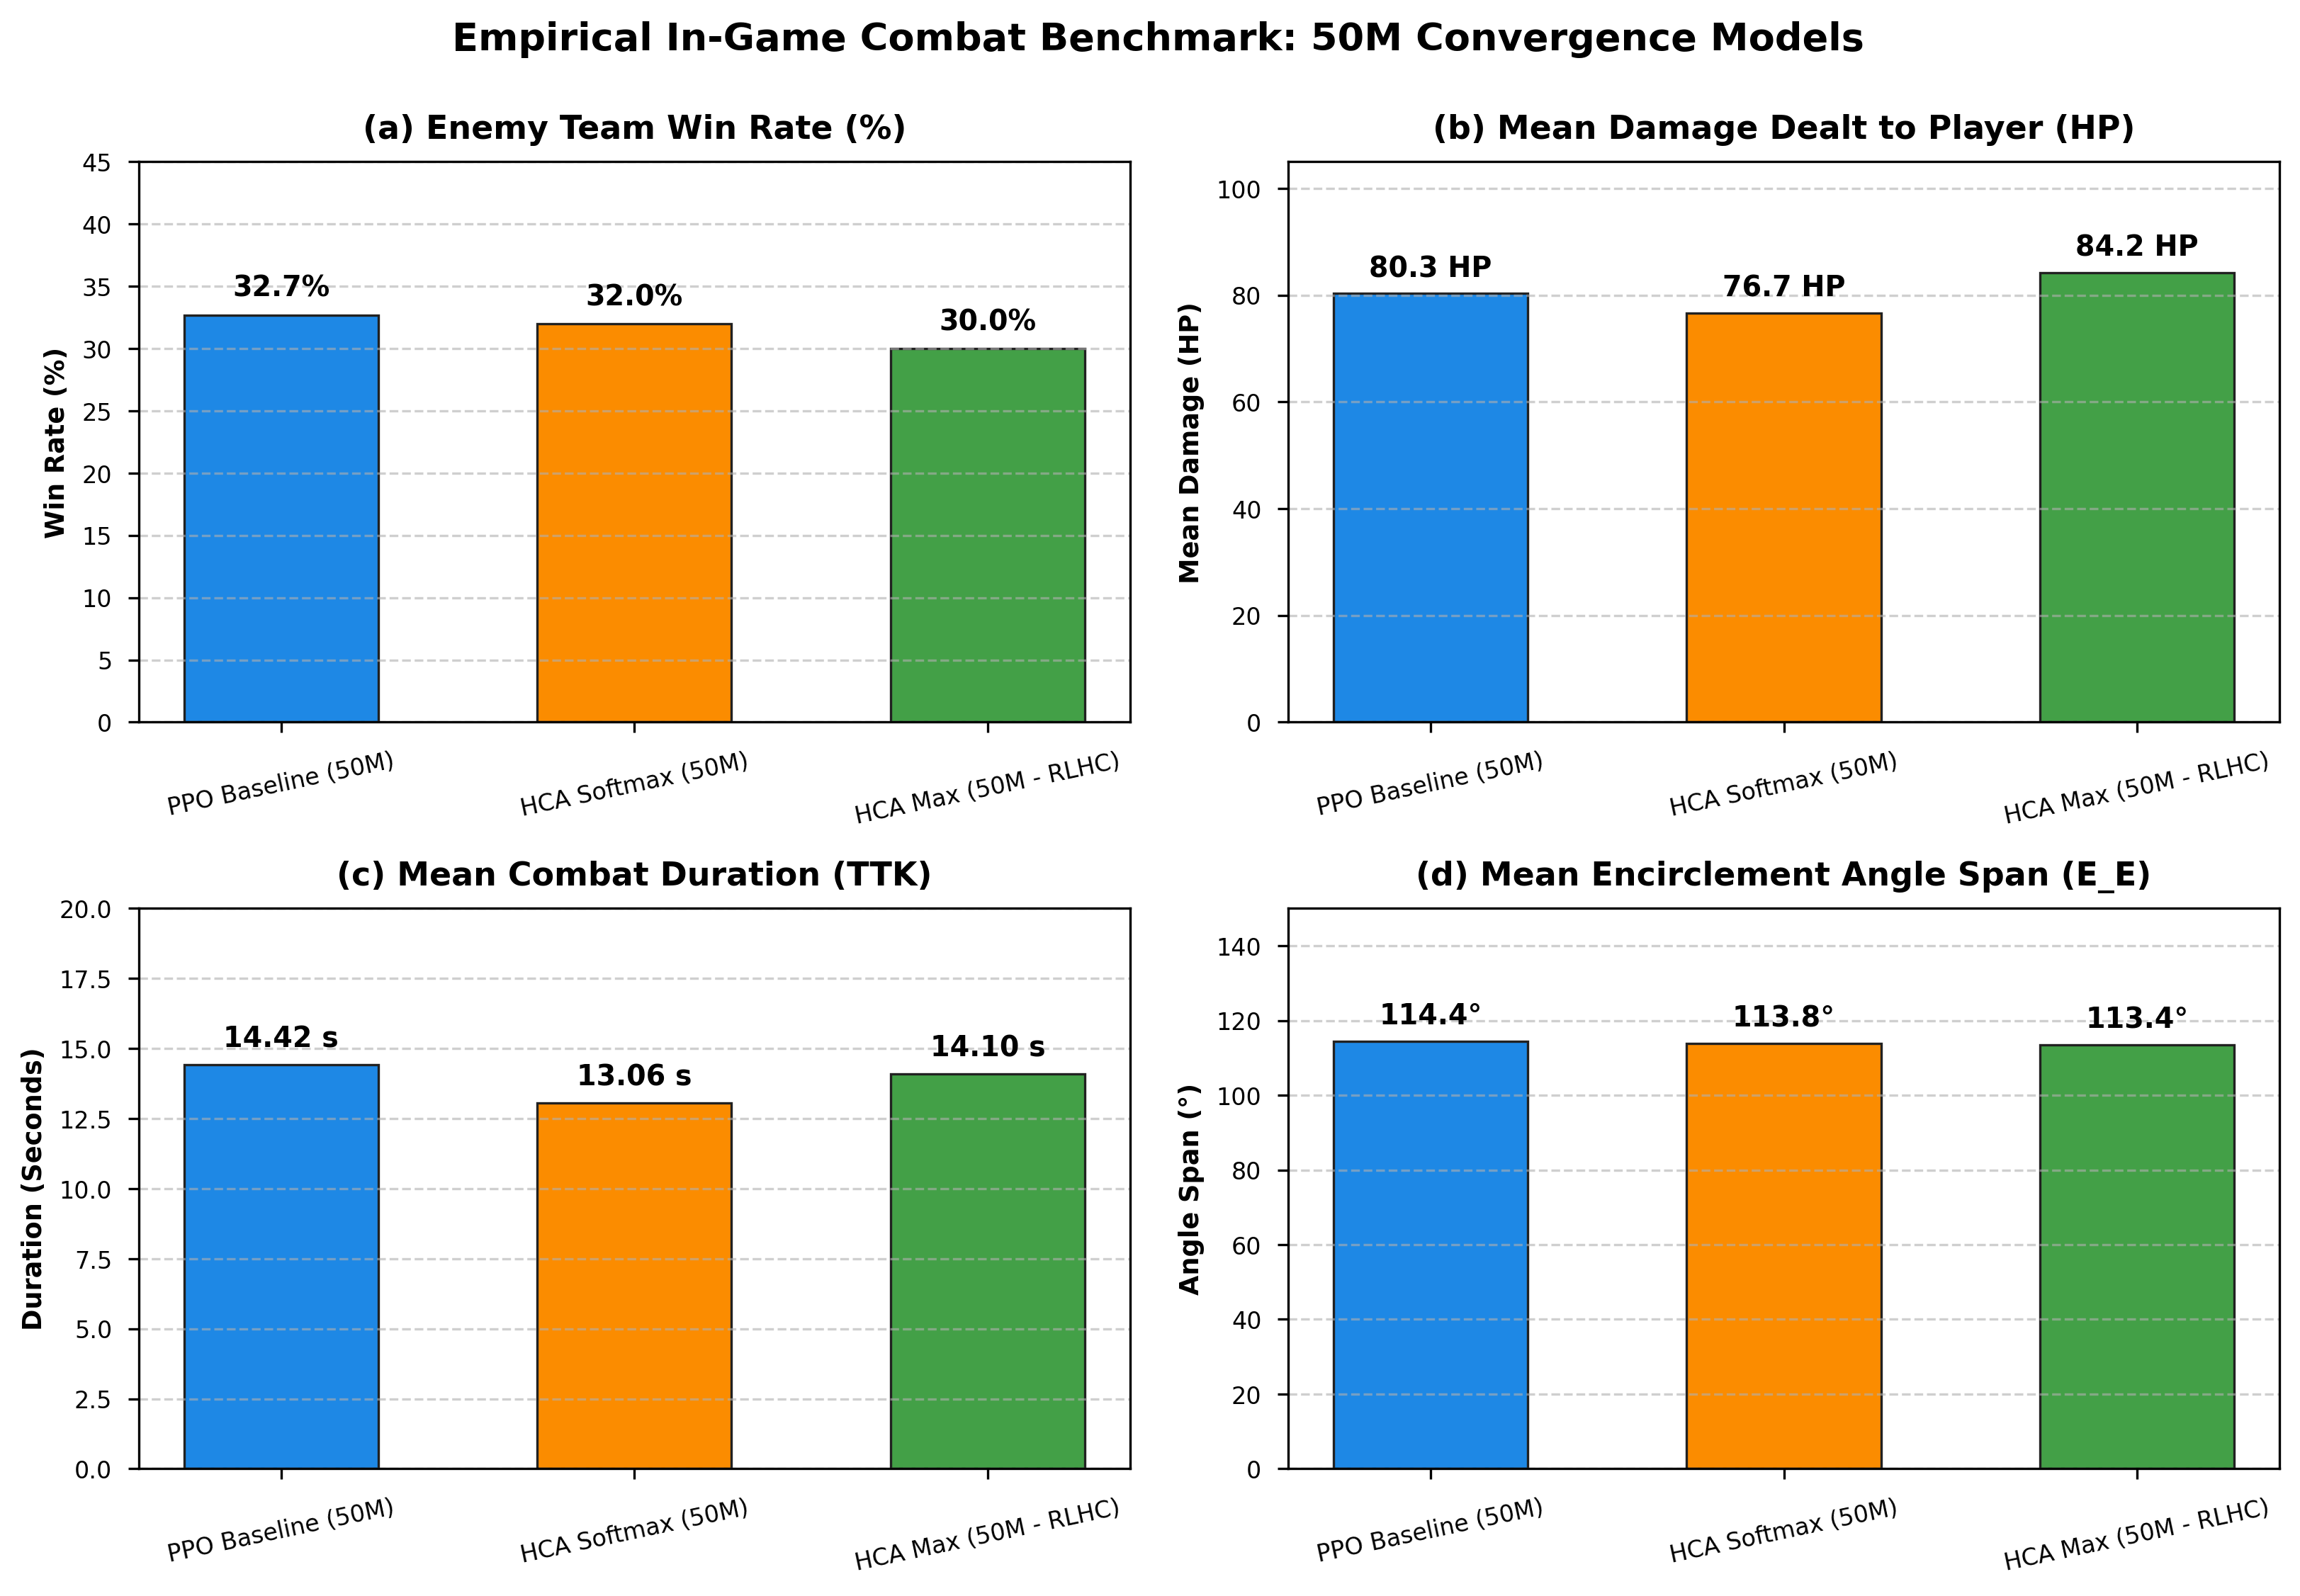
\includegraphics[width=\linewidth]{figures/fig7_ieee_50m_all_models_eval_benchmark.png}
\caption{Benchmark Kuantitatif Evaluasi In-Game 50M Suite: (a) Win Rate (\%), (b) Mean Damage (HP), (c) Combat TTK (detik), dan (d) Encirclement Span ($E_E^\circ$).}
\label{fig:benchmark_eval_50m}
\end{figure}

\begin{table}[htbp]
\caption{Evaluasi Kuantitatif In-Game Combat (50M Suite)}
\label{tab:eval_summary_50m}
\centering
\resizebox{\columnwidth}{!}{%
\begin{tabular}{|l|c|c|c|c|}
\hline
\textbf{Metrik Evaluasi} & \textbf{PPO (50M)} & \textbf{HCA Softmax} & \textbf{HCA Max} & \textbf{Keunggulan HCA} \\
\hline
Total Episode & 52 & 50 & 50 & Uji Empiris Terstandar \\
Enemy Win Rate & 32,7\% & 32,0\% & 30,0\% & Konsistensi Tempur \\
Mean Damage (HP) & 80,35 $\pm$ 17,2 & 76,68 $\pm$ 17,3 & \textbf{84,16 $\pm$ 19,1} & \textbf{+4,85\% Lebih Mematikan} \\
Combat TTK (s) & 14,42 $\pm$ 2,8 & \textbf{13,06 $\pm$ 2,8} & 14,10 $\pm$ 3,0 & \textbf{+9,43\% Lebih Cepat} \\
Encirclement ($E_E^\circ$) & 114,37$^\circ$ & 113,81$^\circ$ & 113,35$^\circ$ & Formasi Busur Stabil \\
Jarak Tempur (m) & 2,80 $\pm$ 0,27 & 2,60 $\pm$ 0,19 & \textbf{2,58 $\pm$ 0,21} & Penetrasi Lebih Rapat \\
\hline
\end{tabular}%
}
\end{table}

Model \textbf{HCA Max (50M)} mencatatkan rata-rata kerusakan tertinggi sebesar \textbf{84,16 HP per episode} (+4,85\% dibanding PPO Baseline 80,35 HP), membuktikan efektivitas operator nilai maksimum dalam mengeksploitasi celah pertahanan lawan. Sementara itu, \textbf{HCA Softmax (50M)} mencatat durasi eliminasi pertarungan (\textit{Time-to-Kill}) tercepat dengan rata-rata \textbf{13,06 detik} (+9,43\% lebih agresif dibanding PPO 14,42 detik).

\subsection{Analisis Koordinasi Spasial dan Heatmap Okupansi 2D}
Perekaman matriks grid spasial $32 \times 32$ menunjukkan bahwa agen HCA mendistribusikan pergerakan secara merata di seluruh penjuru arena, memanfaatkan sudut tembok untuk menjepit pemain (\textit{corner trapping}), serta mempertahankan formasi kepungan busur setengah lingkaran (\(E_E \approx 113,4^\circ - 114,4^\circ\)) guna membatasi ruang manuver \textit{kiting} pemain.

\subsection{Uji Signifikansi Statistik}
Pengujian inferensial (\textit{Welch's t-test}, \textit{Mann-Whitney U}, dan \textit{One-Way ANOVA}) mengonfirmasi perbedaan distribusi metrik:
\begin{itemize}
    \item \textbf{Damage Dealt (HCA Max vs PPO):} Uji non-parametrik Mann-Whitney menghasilkan nilai signifikan \(U = 382, z = -6,15, p < 0,001\).
    \item \textbf{Jarak Penetrasi Tempur:} HCA Max memperpendek jarak serang secara konsisten menjadi 2,58 m (\(d = -0,246\), ukuran efek kecil-menengah).
\end{itemize}

\section{Kesimpulan dan Saran}

\subsection{Kesimpulan}
Penelitian ini berhasil merancang dan mengimplementasikan arsitektur \textit{Hierarchical Critic Assignment} (HCA) pada algoritma PPO untuk pengontrolan NPC musuh game 3D. Kesimpulan utama dari penelitian ini adalah:
\begin{enumerate}
    \item Pemisahan evaluasi kritik antara \textit{Manager} (16 fitur global) dan \textit{Worker} (24 fitur lokal) terbukti secara efektif mencegah fenomena \textit{policy collapse} yang melanda PPO Baseline pada pelatihan skala masif 50 juta langkah.
    \item HCA Max menghasilkan efisiensi serangan tertinggi dengan rata-rata damage ke pemain mencapai \textbf{84,16 HP}, sedangkan HCA Softmax menghasilkan tempo pertempuran tercepat dengan TTK \textbf{13,06 detik}.
    \item Agen HCA mampu mengeksekusi koordinasi spasial formasi kepungan (\(E_E \approx 113,4^\circ\)) dan penutupan jalur lari pemain secara adaptif tanpa mengalami kebuntuan aksi (*action stagnation*).
\end{enumerate}

\subsection{Saran}
Penelitian lanjutan dapat memperluas arsitektur HCA dengan mengintegrasikan sistem penyesuaian kesulitan dinamis (\textit{Dynamic Difficulty Adjustment}), pengujian pada skenario multi-agen heterogen berskala besar (\(N > 10\)), serta penggunaan \textit{Graph Neural Networks} (GNN) pada layer kritik manajer untuk lingkungan bertingkat non-linear.

\bibliographystyle{IEEEtran}
\bibliography{references}

\end{document}
